% !TEX program = xelatex
% Cards format — auto-generated from kidlisp-cards.tex by cards-convert.mjs
\documentclass[11pt]{article}

\usepackage{fontspec}
\usepackage{unicode-math}
\setmainfont{Latin Modern Roman}
\setsansfont{Latin Modern Sans}
\setmonofont{Latin Modern Mono}[Scale=0.88]


\usepackage{graphicx}
\graphicspath{{figures/}{../arxiv-kidlisp/figures/}}
\usepackage{booktabs}
\usepackage{tabularx}
\usepackage{ragged2e}
\usepackage{microtype}
\usepackage{natbib}
\usepackage{listings}

\newfontfamily\kidlispbold{ywft-processing-bold}[
  Path=../../system/public/type/webfonts/,
  Extension=.ttf
]
\newfontfamily\kidlispfont{ywft-processing-light}[
  Path=../../system/public/type/webfonts/,
  Extension=.ttf
]
\lstdefinelanguage{kidlisp}{
  morekeywords=[1]{wipe,ink,line,box,circle,tri,plot,flood,shape,zoom,scroll,spin,blur,contrast,embed,layer,width,height,frame,time,wiggle,melody,mic,suck,sort,form,trans,cube,move,scale,hop,overtone,resolution,write,text,type,stamp,paste,point,poly,noise,fade,pan,unpan,mask,unmask,flip,crawl,left,right,up,down,goto,face,outline,fill,stroke},
  morekeywords=[2]{def,let,if,cond,once,later,lambda,do},
  morekeywords=[3]{repeat},
  morekeywords=[4]{random,sin,cos,tan,floor,ceil,round,abs,sqrt,min,max},
  sensitive=true,
  morecomment=[l]{;},
  morestring=[b]",
  escapeinside={|}{|},
}
\lstset{
  language=kidlisp,
  basicstyle=\ttfamily\small,
  keywordstyle=[1]\color{klfn}\bfseries,
  keywordstyle=[2]\color{klform}\bfseries,
  keywordstyle=[3]\color{klrepeat}\bfseries,
  keywordstyle=[4]\color{klmath},
  commentstyle=\color{klcmt}\itshape,
  stringstyle=\color{klstr},
  breaklines=true,
  frame=single,
  rulecolor=\color{acgray!30},
  backgroundcolor=\color{acgray!5},
  xleftmargin=0.5em,
  xrightmargin=0.5em,
  aboveskip=0.5em,
  belowskip=0.5em,
}
\lstdefinelanguage{python}{
  morekeywords={def,return,import,from,class,if,else,for,in,with,as,try,except,None,True,False,self,and,or,not,lambda,yield,pass,break,continue,raise,while},
  sensitive=true,
  morecomment=[l]{\#},
  morestring=[b]",
  morestring=[b]',
}
\lstset{
  language=kidlisp,
}

\makeatletter
\def\input@path{{../}}
\makeatother
\usepackage{ac-paper-cards}

% Extra commands from base paper
\newcommand{\kn}[1]{\textcolor{klnum}{#1}}
\newcommand{\kt}[1]{\textcolor{klstr}{#1}}
\newcommand{\kv}[1]{\textcolor{klvar}{#1}}
\newcommand{\ke}[1]{\textcolor{klembed}{\textbf{#1}}}
\newcommand{\km}[1]{\textcolor{klmath}{#1}}
\newcommand{\kidlisp}{\textsc{KidLisp}}
\definecolor{klbrand}{RGB}{205,92,155}
\definecolor{klcyan}{RGB}{112,214,255}
\definecolor{kldark}{RGB}{48,43,58}
\definecolor{klfn}{RGB}{0,136,170}
\definecolor{klform}{RGB}{119,51,170}
\definecolor{klrepeat}{RGB}{170,0,170}
\definecolor{klnum}{RGB}{204,0,102}
\definecolor{klstr}{RGB}{170,120,0}
\definecolor{klcmt}{RGB}{102,102,102}
\definecolor{klmath}{RGB}{0,136,0}
\definecolor{klvar}{RGB}{204,102,0}
\definecolor{klembed}{RGB}{0,136,0}

\hypersetup{
  pdftitle={KidLisp Cards: Programs That Fit on a Card},
}

\renewcommand{\acpdfbase}{kidlisp-cards-26-arxiv}
\begin{document}

% ============================================================
% TITLE CARD
% ============================================================
\thispagestyle{empty}
\vspace*{\fill}
\begin{center}

\includegraphics[height=8em]{pals}\par\vspace{0.3em}
{\acbold\fontsize{20pt}{24pt}\selectfont\color{acdark} Kid{\color{acpurple}Lisp} Cards}\par
\vspace{0.3em}
\vspace{0.5em}
{\normalsize\color{cyan!70!blue}\textbf{@jeffrey}}\par
{\small\color{acgray} Aesthetic.Computer}\par
{\small\color{acgray} ORCID: \href{https://orcid.org/0009-0007-4460-4913}{0009-0007-4460-4913}}\par
\vspace{0.8em}
\rule{0.6\textwidth}{1pt}\par
\vspace{0.4em}
{\small\color{acpink!40}\textit{working draft --- not for citation}}\par
\vspace{0.3em}
{\footnotesize\color{acgray} March 2026}\par
\end{center}
\vspace*{\fill}

% ============================================================
% INDEX CARD
% ============================================================
\cardindex

% ============================================================
% BODY
% ============================================================
\section{Introduction}

Most programming languages produce programs that are too long to print on an index card. This is a consequence of abstraction: general-purpose languages encourage decomposition into functions, classes, modules, and files. The program is distributed across a codebase. No single artifact captures the whole.

\kidlisp{} is different. Its programs are typically 1--6 lines long. A complete animated scene, a geometric pattern, a recursive fractal, or a moiré interference pattern fits in a few S-expressions. This is not a limitation but a design choice: \kidlisp{} omits user-defined functions, recursion (except through \texttt{later}), mutable data structures, and imports. Programs are flat sequences of drawing commands, loops, and conditionals.

This flatness creates an opportunity. If the source code of a program fits on a card, and the visual output of that program fits on the same card, then the card becomes a self-contained artifact: a program you can hold, pass to someone, pin to a wall, or mail. The card is both documentation and executable. It is a \emph{score}---instructions for producing a visual event.

This paper describes the KidLisp Cards format (\S\ref{sec:format}), the offline rendering pipeline (\S\ref{sec:pipeline}), the current card catalog (\S\ref{sec:catalog}), layout variations and their social and physical affordances (\S\ref{sec:layouts}), and speculative futures for the format (\S\ref{sec:futures}).

% ============ 2. THE CARD FORMAT ============

\section{The Card Format}
\label{sec:format}

A KidLisp Card has three elements:

\begin{enumerate}
  \item \textbf{Title.} A short name that evokes the visual output: ``Starburst,'' ``Honeycomb,'' ``Spiral Walk.''
  \item \textbf{Rendered output.} A pixel-art image (160$\times$120 default resolution, upscaled 3$\times$ with nearest-neighbor interpolation to preserve hard edges).
  \item \textbf{Source code.} The complete \kidlisp{} program, typically 1--4 lines, displayed in monospace below the image.
\end{enumerate}

The card is self-contained: anyone who reads the source code can reproduce the image exactly, in any \kidlisp{} interpreter. There are no external dependencies, no imports, no configuration. The program \emph{is} the card.

\subsection{Card Dimensions}

The rendered image occupies a 160$\times$120 pixel canvas (4:3 ratio), matching the default \kidlisp{} resolution. At 3$\times$ upscale, this produces a 480$\times$360 pixel image suitable for screen display. For print, cards are sized at 4$\times$6 inches (standard index card / postcard), with the image occupying the upper portion and the source code below.

\subsection{What Makes a Good Card}

Not every \kidlisp{} program makes a good card. The best cards share properties:

\begin{itemize}
  \item \textbf{Brevity.} 1--4 lines. If the source code doesn't fit comfortably below the image, the program is too long for the format.
  \item \textbf{Surprise.} The output should be more complex or beautiful than the source code suggests. A three-line program that produces a moiré pattern rewards inspection.
  \item \textbf{Legibility.} A reader should be able to trace from source to output without running the program. The connection between code and image should be discernible, even if not immediately obvious.
  \item \textbf{Independence.} No \texttt{\$code} embeds, no external state. The card must work in isolation.
\end{itemize}

\begin{figure}[t]
\centering
\fbox{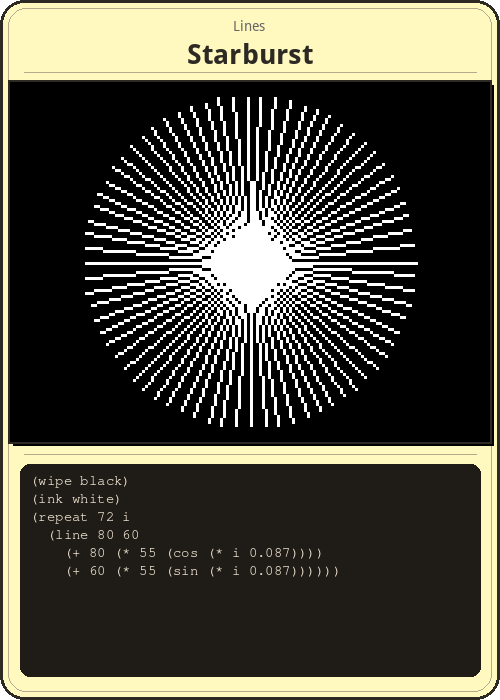
\includegraphics[width=0.47\columnwidth]{card-starburst.png}}%
\hfill%
\fbox{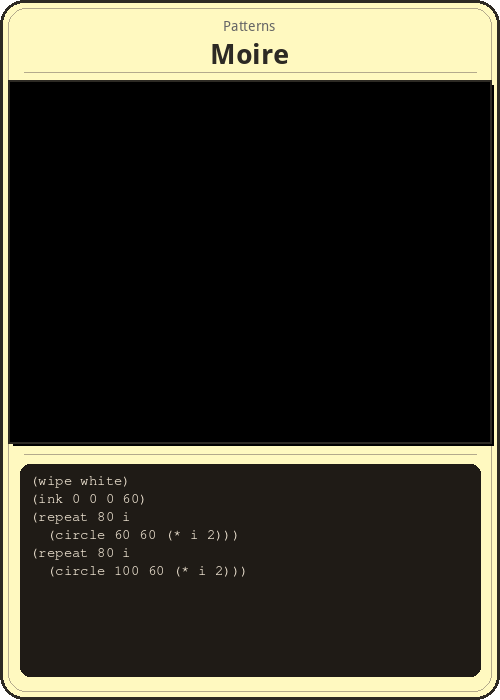
\includegraphics[width=0.47\columnwidth]{card-moire.png}}
\caption{Two program cards rendered by the Python interpreter: ``Starburst'' (72 radial lines, 3 lines of code) and ``Moir\'{e}'' (overlapping concentric circles, 3 lines). These are trivial examples---they demonstrate the card format's structure but do not represent the expressive range of the language or the ambitions of the format.}
\label{fig:program-cards}
\end{figure}

% ============ 3. RENDERING PIPELINE ============

\section{Offline Rendering Pipeline}
\label{sec:pipeline}

KidLisp Cards are rendered using a Python interpreter that runs outside the browser. This enables batch rendering, print production, and notebook-based curation without requiring the full Aesthetic Computer runtime.

\subsection{The Python Interpreter}

The interpreter (\texttt{notebooks/ac.py}, 452 lines) implements a subset of \kidlisp{} sufficient for static card rendering:

\begin{itemize}
  \item \textbf{Drawing:} \texttt{wipe}, \texttt{ink}, \texttt{line}, \texttt{box}, \texttt{circle}, \texttt{tri}, \texttt{plot}, \texttt{shape}, \texttt{flood}
  \item \textbf{Turtle:} \texttt{crawl}, \texttt{left}, \texttt{right}, \texttt{goto}, \texttt{face}, \texttt{up}, \texttt{down}
  \item \textbf{Control:} \texttt{repeat}, \texttt{if}, \texttt{def}, \texttt{later}, \texttt{do}
  \item \textbf{Math:} full arithmetic, trigonometry, \texttt{abs}, \texttt{sqrt}, \texttt{min}, \texttt{max}
  \item \textbf{Canvas:} \texttt{resolution}, \texttt{fill}, \texttt{outline}, \texttt{stroke}
\end{itemize}

The interpreter uses PIL (Pillow) for rendering. Each card is drawn on an RGBA canvas, upscaled with nearest-neighbor interpolation, and exported as PNG. The Python implementation is intentionally simpler than the browser evaluator (15,161 lines)---it omits animation, audio, embedding, and timing syntax, focusing only on the subset needed for static visual output.

\subsection{Jupyter Notebook Workflow}

The primary curation tool is a Jupyter notebook (\texttt{notebooks/kidlisp-cards.ipynb}). The \texttt{show\_card()} function renders a program and displays it inline as an HTML card:

\begin{lstlisting}[language=python,basicstyle=\ttfamily\footnotesize]
show_card("Starburst", """(wipe black)
(ink white)
(repeat 72 i
  (line 80 60
    (+ 80 (* 55 (cos (* i 0.087))))
    (+ 60 (* 55 (sin (* i 0.087))))))""")
\end{lstlisting}

Each call produces a dark-background card with the title, rendered image, and source code displayed inline. The notebook serves as both a development environment and a gallery---scrolling through the notebook is like flipping through a deck of cards.

\subsection{Two Interpreters, One Language}

The existence of two independent interpreters (JavaScript in the browser, Python in the notebook) serves as a cross-validation mechanism. If a program renders identically in both, its behavior is determined entirely by the language semantics rather than implementation details. Programs that rely on browser-specific features (animation, audio, embedded layers) are excluded from the card format by construction---they simply won't render in the Python interpreter.

% ============ 4. CARD CATALOG ============

\section{The Card Catalog}
\label{sec:catalog}

The current notebook contains 28 cards organized into seven categories. Each category explores a different aspect of the language through minimal examples. These programs are deliberately trivial---drawing exercises, mathematical illustrations, turtle walks. They establish the card format's structure but do not represent its expressive potential. The interesting cards have not been made yet. The format's value will emerge from programs that use brevity to say something worth saying, not from geometric demos.

\subsection{Lines}

Line cards demonstrate \texttt{repeat} and trigonometry. A starburst radiates 72 lines from center. A crosshatch overlays horizontal and vertical grids at low opacity.

\begin{figure}[h]
\centering
\fbox{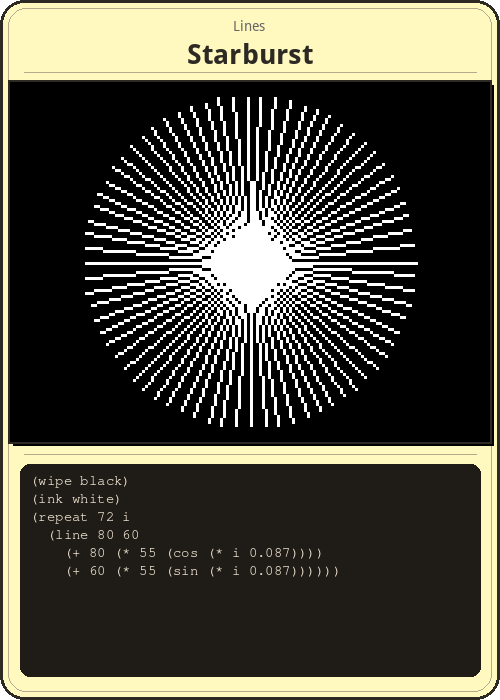
\includegraphics[width=0.47\columnwidth]{card-starburst.png}}%
\hfill%
\fbox{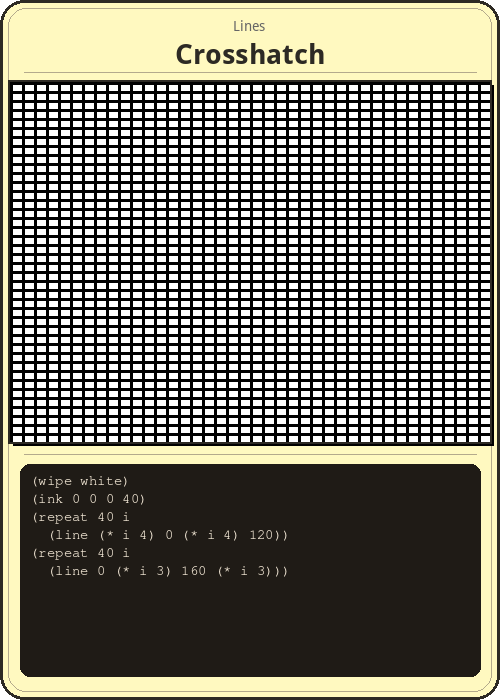
\includegraphics[width=0.47\columnwidth]{card-crosshatch.png}}
\caption{``Starburst'' and ``Crosshatch'' --- line cards.}
\label{fig:lines}
\end{figure}

\begin{lstlisting}
; Starburst — 72 radial lines
(wipe |\kt{black}|)
(ink |\kt{white}|)
(repeat |\kn{72}| |\kv{i}|
  (line |\kn{80}| |\kn{60}|
    (|\km{+}| |\kn{80}| (|\km{*}| |\kn{55}| (|\km{cos}| (|\km{*}| |\kv{i}| |\kn{0.087}|))))
    (|\km{+}| |\kn{60}| (|\km{*}| |\kn{55}| (|\km{sin}| (|\km{*}| |\kv{i}| |\kn{0.087}|))))))
\end{lstlisting}

\subsection{Circles}

Circle cards use \texttt{outline} mode and nested \texttt{repeat} loops. ``Ripple'' draws 30 concentric circles with blue-shifting color.

\begin{figure}[h]
\centering
\fbox{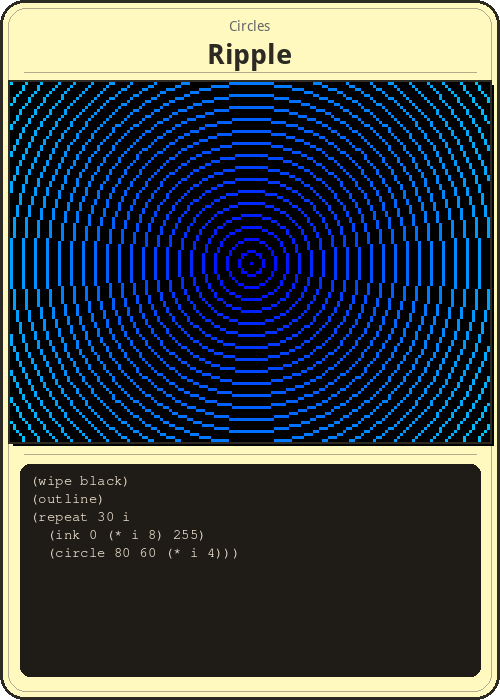
\includegraphics[width=0.47\columnwidth]{card-ripple.png}}%
\hfill%
\fbox{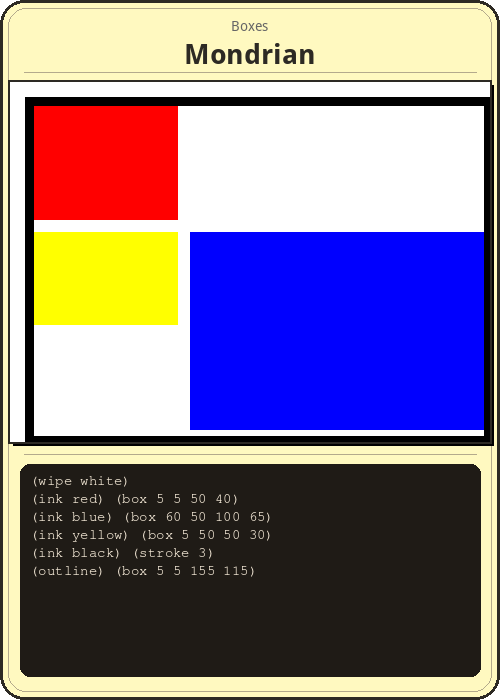
\includegraphics[width=0.47\columnwidth]{card-mondrian.png}}
\caption{``Ripple'' (circles) and ``Mondrian'' (boxes).}
\label{fig:circles-boxes}
\end{figure}

\subsection{Boxes \& Composition}

``Mondrian'' recreates the primary-color grid with four colored rectangles. ``Nest'' draws 10 inset rectangles with shifting hues.

\subsection{Math \& Curves}

These cards use \texttt{plot} with mathematical functions. ``Lissajous'' draws a Lissajous figure with 600 points. ``Spiral'' plots a polar spiral.

\begin{figure}[h]
\centering
\fbox{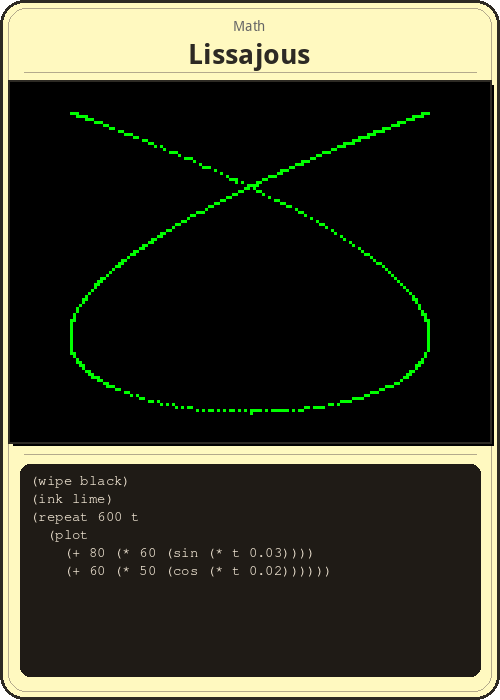
\includegraphics[width=0.47\columnwidth]{card-lissajous.png}}%
\hfill%
\fbox{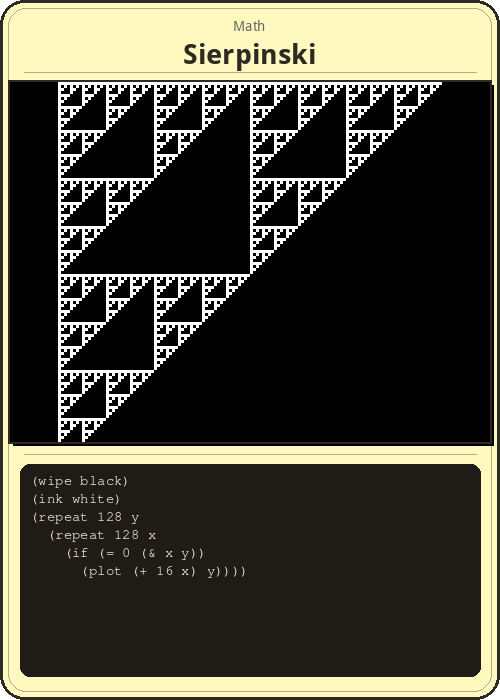
\includegraphics[width=0.47\columnwidth]{card-sierpinski.png}}
\caption{``Lissajous'' (math curves) and ``Sierpinski'' (bitwise AND fractal).}
\label{fig:math}
\end{figure}

\subsection{Color \& Gradients}

``Sierpinski'' uses bitwise AND to generate the Sierpinski triangle: \texttt{(if (= 0 (\& x y)) (plot (+ 16 x) y))}. ``Sunflower'' plots 500 points along a golden-angle spiral with cycling colors.

\subsection{Turtle Graphics}

Turtle cards use \texttt{crawl}, \texttt{left}, \texttt{right}, and \texttt{face}. A five-pointed star uses \texttt{(right 144)}. A tree uses \texttt{later} for recursive branching. A snowflake nests Koch-curve segments.

\begin{figure}[h]
\centering
\fbox{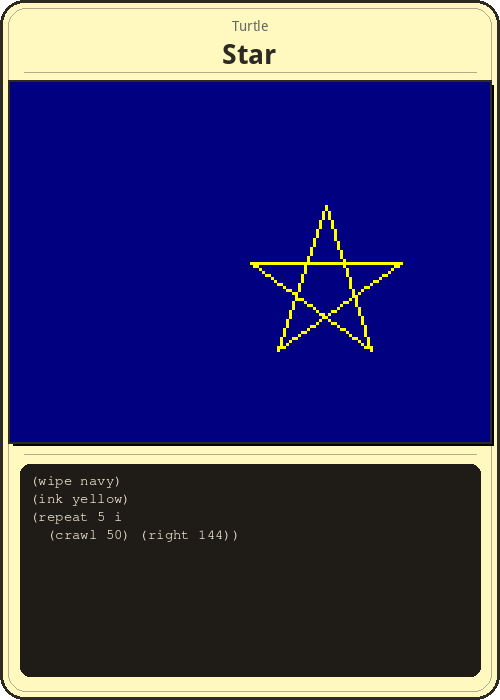
\includegraphics[width=0.47\columnwidth]{card-star.png}}%
\hfill%
\fbox{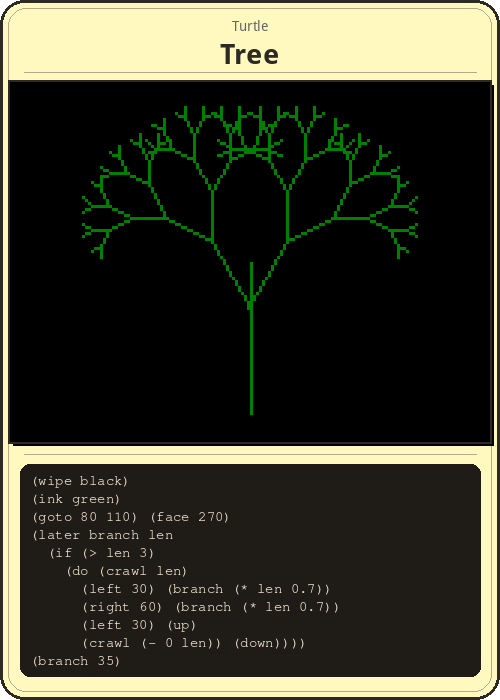
\includegraphics[width=0.47\columnwidth]{card-tree.png}}
\caption{``Star'' and ``Tree'' --- turtle graphics cards.}
\label{fig:turtle}
\end{figure}

\begin{lstlisting}
; Star — 5 sides, 144-degree turns
(wipe |\kt{navy}|)
(ink |\kt{yellow}|)
(repeat |\kn{5}| |\kv{i}| (crawl |\kn{50}|) (right |\kn{144}|))
\end{lstlisting}

\subsection{Minimal Koans}

The shortest cards in the deck. ``Horizon'' is three lines: dark sky, gold earth. ``Pip'' is a single red dot on black. These cards approach the minimum viable program---the smallest amount of code that produces a recognizable image.

\begin{figure}[h]
\centering
\fbox{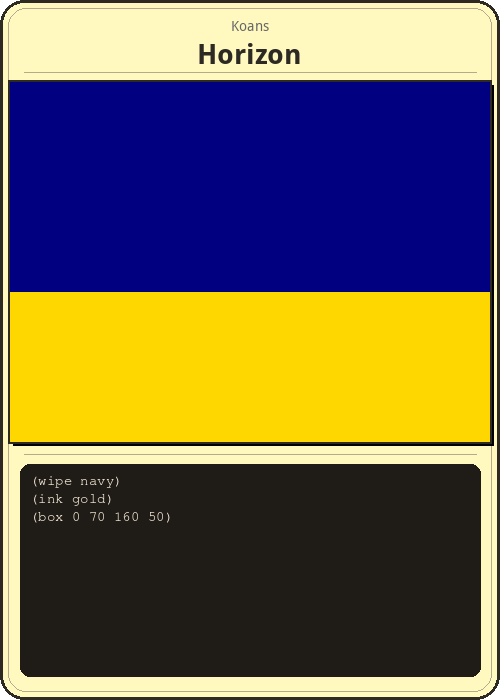
\includegraphics[width=0.47\columnwidth]{card-horizon.png}}%
\hfill%
\fbox{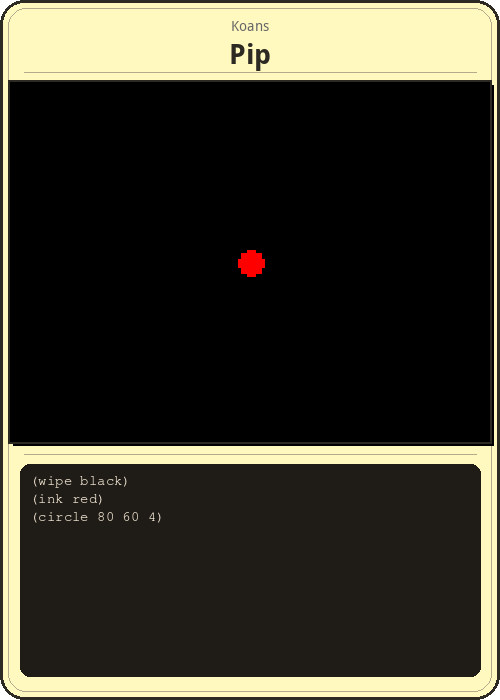
\includegraphics[width=0.47\columnwidth]{card-pip.png}}
\caption{``Horizon'' and ``Pip'' --- minimal koans (2--3 lines each).}
\label{fig:koans}
\end{figure}

\begin{lstlisting}
; Pip — the minimum card
(wipe |\kt{black}|)
(ink |\kt{red}|)
(circle |\kn{80}| |\kn{60}| |\kn{4}|)
\end{lstlisting}

\begin{figure*}[t]
\centering
\fbox{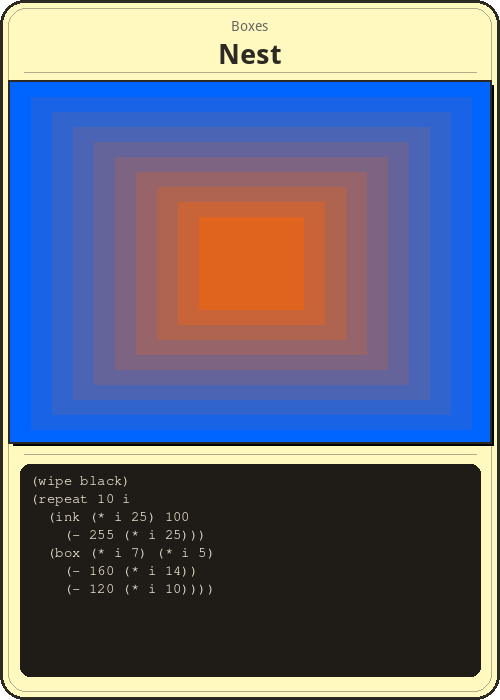
\includegraphics[height=5.5cm]{card-nest.png}}%
\hfill%
\fbox{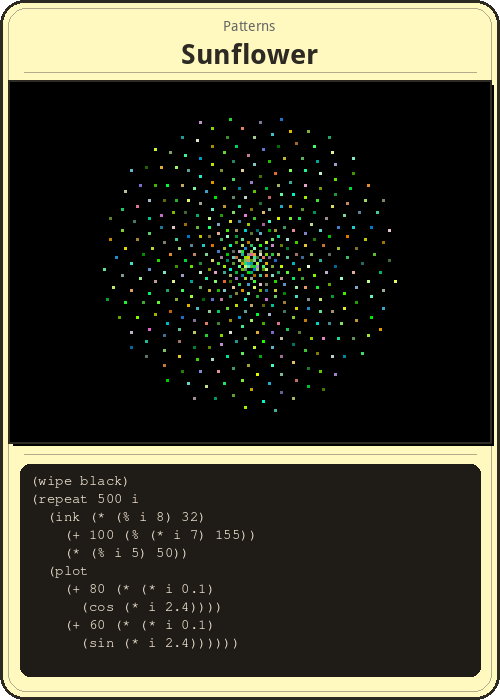
\includegraphics[height=5.5cm]{card-sunflower.png}}%
\hfill%
\fbox{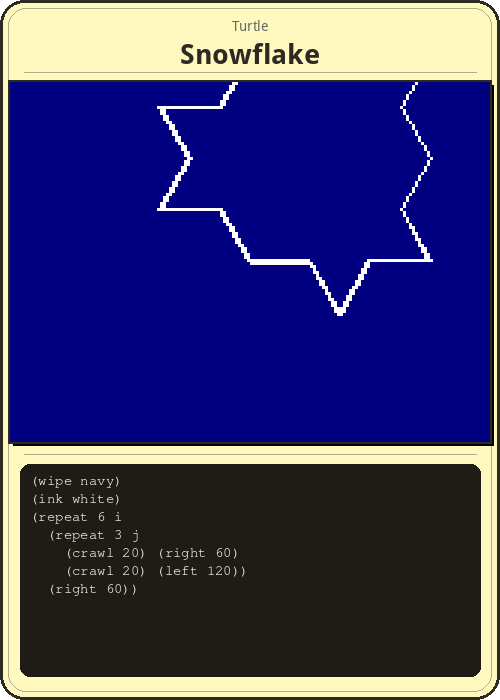
\includegraphics[height=5.5cm]{card-snowflake.png}}%
\hfill%
\fbox{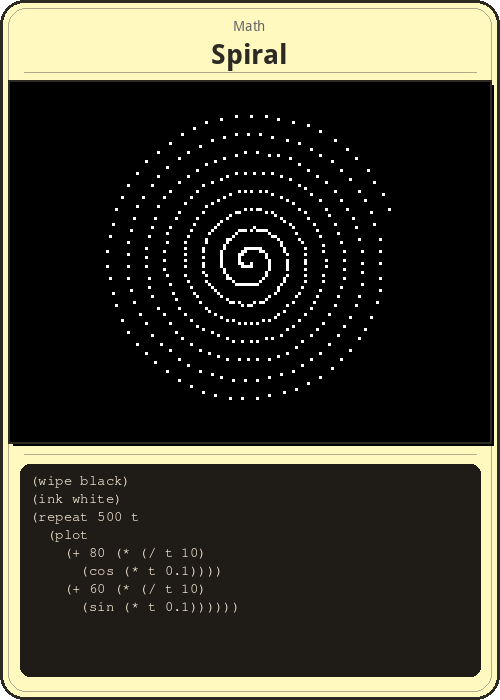
\includegraphics[height=5.5cm]{card-spiral.png}}
\caption{Four complete cards showing the format: title, rendered output, and source code. Left to right: ``Nest,'' ``Sunflower,'' ``Snowflake,'' ``Spiral.'' Each card is self-contained---the source code below the image is the complete program. These are trivial drawing exercises, not expressions of the format's potential.}
\label{fig:four-cards}
\end{figure*}

% ============ 5. LAYOUTS ============

\section{Layouts}
\label{sec:layouts}

The card format has no fixed layout. How the three elements (title, output, source) are arranged determines what the card affords---what you can do with it physically and socially. This section explores layout variations and their consequences.

\begin{figure*}[t]
\centering
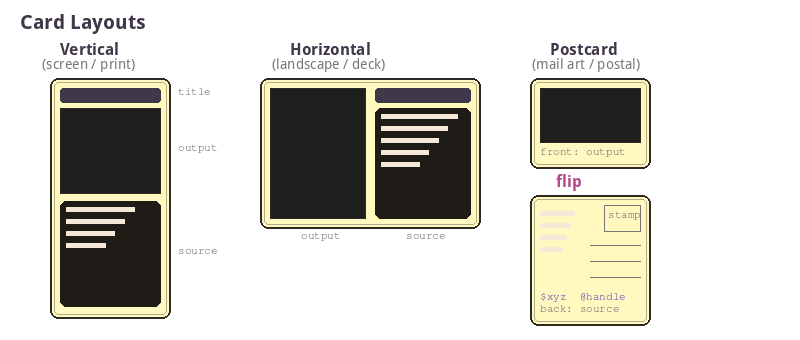
\includegraphics[width=\textwidth]{layout-comparison.png}
\caption{Three layout strategies. \textbf{Vertical:} title / image / source stacked top-to-bottom, optimized for phone screens and portrait printing. \textbf{Horizontal:} image on the left, title and source on the right, suited for landscape cards and side-by-side deck browsing. \textbf{Postcard:} rendered output on the front, source code and metadata on the back---a mailable card where the program is hidden until you flip it over.}
\label{fig:layouts}
\end{figure*}

\subsection{Vertical (Screen / Print)}

The default layout stacks title, image, and source top-to-bottom. This is the notebook layout---it scrolls naturally on a phone or in a Jupyter notebook. For print, it maps to a 4$\times$6 inch card in portrait orientation. The reader's eye moves downward from name to image to code, tracing the relationship between the program and its output.

\subsection{Horizontal (Deck / Landscape)}

A landscape layout places the rendered image on the left and the source code on the right. This works for fanning cards across a table, for slide decks, and for side-by-side comparison. Two cards placed next to each other create a diptych---the viewer can compare programs and outputs simultaneously.

\subsection{Postcard (Mail Art)}

The postcard layout separates front from back. The front shows only the rendered image, full-bleed, no text. The back shows the source code, the author's handle, the short code (\texttt{\$xyz}), and a stamp area. The recipient sees the image first---a visual artifact. Flipping the card reveals the program: the instructions that produced it. The card is both art object and executable score, depending on which side you read.

\begin{figure*}[h]
\centering
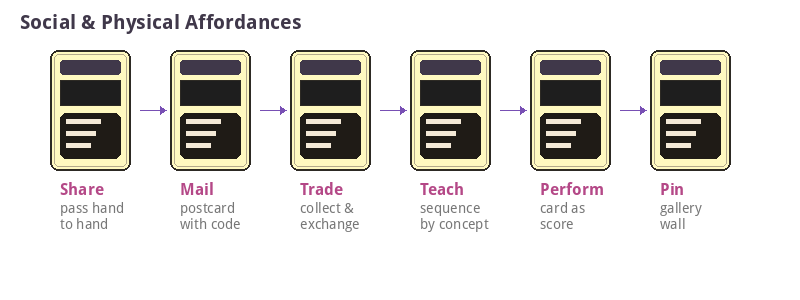
\includegraphics[width=\textwidth]{layout-affordances.png}
\caption{Social and physical affordances of the card format. Each affordance follows from the card's materiality: it can be \textbf{shared} hand-to-hand, \textbf{mailed} as a postcard, \textbf{traded} and collected, \textbf{taught from} in pedagogical sequences, \textbf{performed} as a graphic score, or \textbf{pinned} to a gallery wall.}
\label{fig:affordances}
\end{figure*}

\subsection{Deck Arrangements}

Cards are not single objects. They form decks, and the arrangement of a deck creates meaning. A \emph{pedagogical sequence} orders cards by concept: boxes first (coordinates), then lines (trigonometry), then circles (radius), then math curves, then turtle graphics, then minimal koans. A \emph{gallery grid} arranges cards spatially on a wall, inviting comparison across categories. A \emph{shuffled deck} randomizes the order, producing unexpected juxtapositions between a fractal and a horizon, between a tree and a dot.

\begin{figure}[h]
\centering
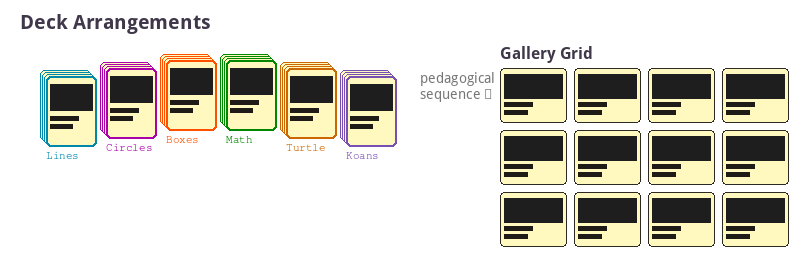
\includegraphics[width=\columnwidth]{layout-decks.png}
\caption{Deck arrangements. Left: cards fanned by category (Lines, Circles, Boxes, Math, Turtle, Koans) with multiple cards stacked per category. Right: a gallery grid where cards are arranged spatially for browsing.}
\label{fig:decks}
\end{figure}

% ============ 6. CARDS IN THE WILD ============

\section{Cards in the Wild}
\label{sec:wild}

The notebook cards are exercises. The real \kidlisp{} corpus---16,000+ programs created by 59 authors---contains pieces that use the full runtime: animation, audio, embedded layers, gradient fades, random placement, and timing syntax. These pieces are short enough for the card format but far more expressive than the notebook examples. Their preview images are rendered by the oven service (Puppeteer-based screenshot capture) and served via CDN.

\begin{figure*}[t]
\centering
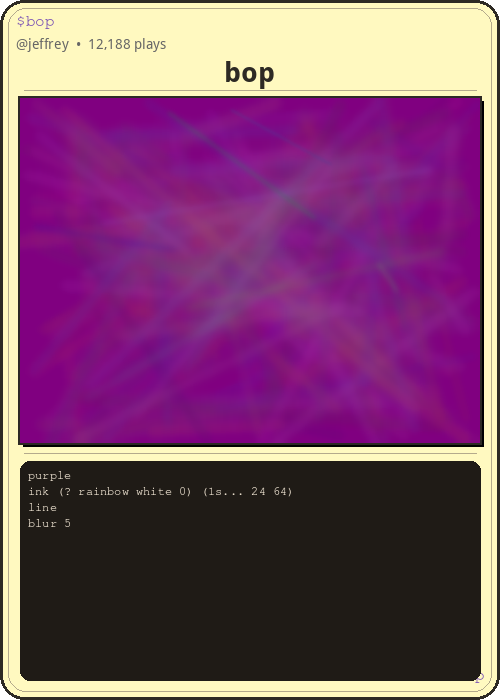
\includegraphics[height=7cm]{user-card-bop.png}%
\hfill%
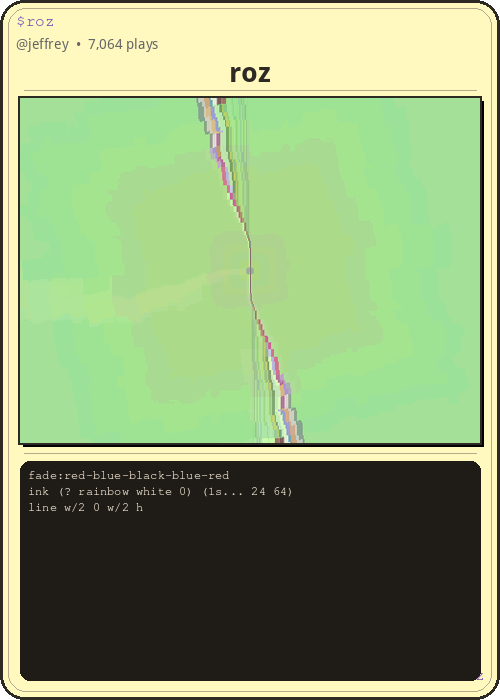
\includegraphics[height=7cm]{user-card-roz.png}%
\hfill%
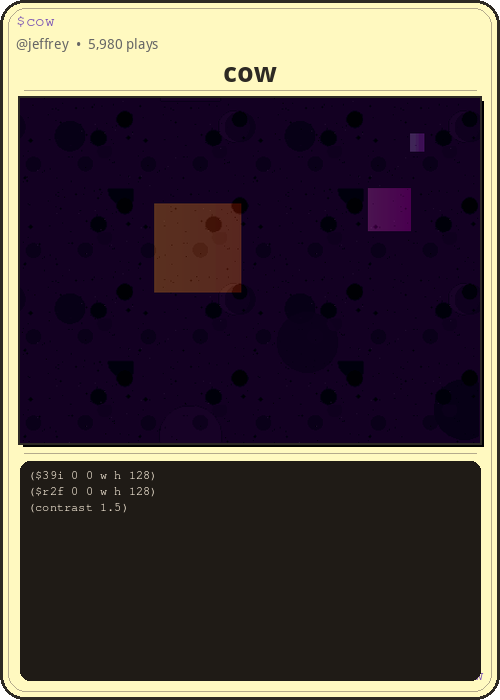
\includegraphics[height=7cm]{user-card-cow.png}%
\hfill%
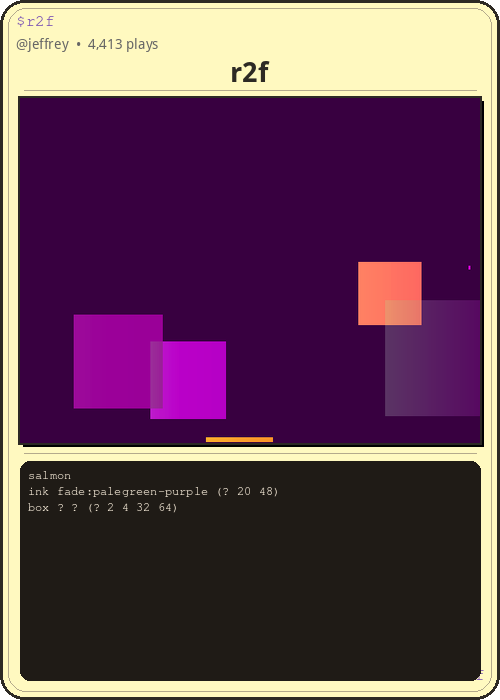
\includegraphics[height=7cm]{user-card-r2f.png}
\caption{Four cards from the live \kidlisp{} corpus, rendered by the oven service. Left to right: \texttt{\$bop} (12,188 plays---the most popular piece, 4 lines), \texttt{\$roz} (7,064 plays, 3 lines), \texttt{\$cow} (5,980 plays---a composition embedding two other pieces via \texttt{\$39i} and \texttt{\$r2f}), \texttt{\$r2f} (4,413 plays, 3 lines of random box placement). All by @jeffrey. These programs use features absent from the Python interpreter---animation, randomness (\texttt{?}), gradient fades (\texttt{fade:}), embedded layers (\texttt{\$code})---but their source code still fits on a card.}
\label{fig:user-cards}
\end{figure*}

\subsection{What Real Pieces Add}

The notebook cards use a static subset of \kidlisp{}. Real pieces on \texttt{kidlisp.com} use the full runtime:

\begin{itemize}
  \item \textbf{Animation.} Programs re-evaluate every frame. \texttt{frame} and \texttt{time} change automatically. A single-frame screenshot captures one moment of a living piece.
  \item \textbf{Randomness.} The \texttt{?} operator produces a random value from a list each frame. \texttt{(ink (? red blue green))} flickers between colors.
  \item \textbf{Gradient fades.} \texttt{fade:red-blue-black} interpolates a multi-stop gradient across the canvas, driven by \texttt{frame} count. One expression replaces pages of manual color math.
  \item \textbf{Embedding.} \texttt{(\$cow)} fetches piece \texttt{cow} from MongoDB, evaluates it in an offscreen buffer, and composites the result. Pieces build on pieces.
  \item \textbf{Timing.} \texttt{1s... (zoom 0.5)} applies a zoom every second. No explicit animation loop.
\end{itemize}

These features keep programs short while dramatically expanding what they can express. \texttt{\$bop}---the most-played piece at 12,188 views---is four lines: a purple background, rainbow-flickering ink, a random line, and a blur. On a card, it looks like a frozen moment of a kinetic painting. In the browser, it is one.

\subsection{The Card as Snapshot}

A card of an animated piece is necessarily incomplete. It captures one frame of a temporal process. This incompleteness is part of the format: the card invites you to type the code and see what it actually does. The static image is a promise. The source code is the fulfillment. The short code (\texttt{\$bop}) is the bridge---type it into \texttt{kidlisp.com} and the card comes alive.

% ============ 7. WHAT CARDS COULD BE ============


\section{What Cards Could Be}
\label{sec:futures}

The card format is young. The current notebook is a proof of concept---28 programs rendered offline. But the correspondence between short programs and physical cards suggests several directions.

\subsection{Trading Cards}

A KidLisp Card is collectible in a way that most software is not. Each card has a name, a visual identity, a short code (\texttt{\$xyz}), and an author. Cards could be printed, numbered, and traded. Rare cards might use obscure language features or produce unexpectedly complex output from minimal code. The ``rarity'' of a card is its information density: how much visual complexity emerges from how few characters.

\subsection{Pedagogical Sequences}

The seven categories in the current notebook suggest a teaching order: start with boxes (simple coordinates), move to lines (trigonometry), circles (radius and repetition), math curves (plot and sine), turtle graphics (relative motion), and finally koans (minimal expression). Each card teaches one concept. A teacher could hand students a physical deck and ask them to reproduce each card, modify it, or create a new card in the same category.

\subsection{Printed Scores}

In music, a score is instructions for producing a temporal event. A KidLisp Card is instructions for producing a visual event. Cards could function as graphic scores in the tradition of Cornelius Cardew, John Cage, and the Fluxus event scores. A performer receives a card, interprets the code (by typing it into \texttt{kidlisp.com}, by reading it aloud, by drawing it by hand), and produces an event. The card is the score. The rendering is one possible realization.

\subsection{Postal Art}

At 4$\times$6 inches, a KidLisp Card is a postcard. The front shows the rendered image. The back shows the source code, the author's handle, and the short code for looking it up online. Mail art with executable content---the recipient can type the code and see the image regenerate on their screen. The physical card and the digital program are the same work in two media.

\subsection{Generative Stationery}

Because the Python interpreter is deterministic and standalone, cards can be batch-rendered for print production without network access. A set of cards could be printed as a booklet, a zine, or a boxed set. The \texttt{cards-convert.mjs} pipeline already produces 4$\times$6 inch PDF cards from the paper format; extending this to include rendered program output alongside source code is a natural next step.

\subsection{Constraint as Generative Principle}

The most interesting consequence of the card format is how it feeds back into the language. Programs that don't fit on a card suggest missing abstractions---or suggest that the program is doing too much. The card constraint encourages economy: find the three-line program that produces the most interesting image. This is a generative constraint in the tradition of Oulipo---arbitrary formal restrictions that produce unexpected creative results.

% ============ 6. RELATED WORK ============

\section{Related Work}

\textbf{Printed code.} The demoscene tradition of ``sizecoding'' (programs under 256 bytes) shares the aesthetic of minimal programs producing maximal output. \kidlisp{} Cards are closer to the ``code poem'' tradition, where the source code itself is read as text alongside its output.

\textbf{Graphic scores.} Cardew's \emph{Treatise} (1967) and Cage's \emph{Notations} (1969) established that visual notation can serve as performance instructions without prescribing a specific realization. KidLisp Cards differ in that they are fully executable---the rendering is deterministic, not open to interpretation. But the card-as-score framing invites reinterpretation: what if you ``play'' the card differently each time?

\textbf{Trading card games.} Games like \emph{Magic: The Gathering} (1993) demonstrated that cards with structured metadata (name, type, rules text, art) create rich combinatorial spaces. KidLisp Cards have natural metadata (title, category, function count, line count, output complexity) that could support similar game mechanics.

\textbf{Computational notebooks.} Jupyter notebooks already combine code and output. The KidLisp Cards notebook is a Jupyter notebook, but with a specific constraint: each cell is a self-contained card rather than a step in a longer computation. The notebook is a gallery, not a narrative.

% ============ 7. CONCLUSION ============

\section{Conclusion}

KidLisp Cards emerge from a simple observation: when programs are short enough, they fit on cards. The card format---title, image, source---makes programs into physical artifacts that can be printed, mailed, collected, taught from, and performed. The Python rendering pipeline enables offline batch production. The seven-category catalog provides a curated entry point into the language.

The format is a work in progress. The current deck of 28 cards is a starting point, not a finished collection. The question is not how many cards to make but which programs deserve to be cards---which three-line compositions produce images worth holding in your hand.

The notebook, interpreter, and card catalog are available at \url{https://github.com/whistlegraph/aesthetic-computer}. Programs can be created and shared at \url{https://kidlisp.com}.

\vspace{0.5em}
\noindent\textbf{ORCID:} \href{https://orcid.org/0009-0007-4460-4913}{0009-0007-4460-4913}

% ============ REFERENCES ============

\bibliographystyle{plainnat}
\bibliography{references}

\end{document}
